\documentclass[11pt,a4paper]{article}
\usepackage[spanish]{babel}
 \usepackage[utf8]{inputenc}
\usepackage{anysize} % Soporte para el comando \marginsize
\usepackage{listings}
%\marginsize{3cm}{2.5cm}{2cm}{2cm}
\usepackage[T1]{fontenc}
\usepackage{times}
%\usepackage[hyphens]{url}
\usepackage{hyperref} 

\usepackage{color}    % aunque tambien puedes usar xcolor
\usepackage{graphicx}		% Inclusión de imágenes
\DeclareGraphicsExtensions{.eps}

\definecolor{gray97}{gray}{.97}
\definecolor{gray75}{gray}{.75}
\definecolor{gray45}{gray}{.45}

\lstdefinestyle{Code} {
     framerule=0pt,aboveskip=0.5cm, 
     framextopmargin=2pt,
     framexbottommargin=2pt,
     framexleftmargin=0.1cm,
     framesep=0pt,
     rulesep=.4pt,
     backgroundcolor=\color{gray97},
     rulesepcolor=\color{black},
     %
     stringstyle=\ttfamily,
     showstringspaces = false,
     basicstyle=\footnotesize\ttfamily,
     commentstyle=\color{gray45},
     keywordstyle=\bfseries,
     breaklines=true
   }
% ... Además hay que agregar esta configuración al paquete url

\author{Sergio Del Castillo}
 \title{Tutorial de Instalación}
\hypersetup{
    colorlinks,%
    citecolor=black,%
    filecolor=black,%
    linkcolor=black,%
    urlcolor=blue
}
 
 \begin{document}
 \maketitle
 \tableofcontents{}
 \newpage
 
\section{Instalación: Pasos Generales}
	\begin{enumerate}
		\item Descomprimir el archivo \textsl{alifecontest-java-0.02.zip}.
		\item Instalar maquina virtual y entorno de desarrollo java de SUN.
		\item Instalar compilador de C/C++ (gcc y g++).
		\item Iniciar el entorno.
	\end{enumerate}

\subsection{Usuarios de Windows}
	\begin{enumerate}
	\item Bajar e instalar \href{http://java.sun.com/javase/downloads/index.jsp}{JDK}
	\footnote{Instalador JDK: http://java.sun.com/javase/downloads/index.jsp} ( versión \begin{math}\geq 1.6\end{math} )
	\item Bajar e instalar \href{http://www.mingw.org/wiki/HOWTO_Install_the_MinGW_GCC_Compiler_Suite}{MINGW}
	\footnote{Pagina Oficial de MINGW: http://www.mingw.org/wiki/HOWTO\_Install\_the\_MinGW\_GCC\_Compiler\_Suite}
	 de la página oficial.
	Pero se lo puede descargar más fácil del siguiente \href{http://sourceforge.net/projects/mingw/files/}{link}
	\footnote{Instalador de MINGW: http://sourceforge.net/projects/mingw/files/}.
El archivo que hay que descargar se llama MinGW-5.1.4.exe y  se encuentra en la sección {\it Automated MinGW Installer}.
Dentro de la instalación, en el tercer paso se pide TILDAR los componentes a instalar, se deben tildar: g++ compiler, Java compiler y MinGW Make.
\item Configurar variable de entorno PATH de windows:para modificar el PATH se debe acceder a  las propiedades del Sistema utilizando alguna de las alternativas:
	\begin{enumerate}
		\item {\bf Vista Clásica:} Inicio \begin{math}\to\end{math} Panel de Control \begin{math}\to\end{math} Sistema.
		\item {\bf Vista por Categorías:} Rendimiento y Mantenimiento \begin{math}\to\end{math} Sistema
	\end{enumerate}

   Luego en el tab  de {\bf Opciones Avanzadas}, hacer click en {\bf Variables de Entorno}, buscar PATH en la sección
        {\bf Variables del Sistema} y hacer click en modificar para editarlo.
        
        Se debe agregar al inicio el directorio donde se encuentran instalados los archivos binarios de java JDK, 
        normalmente se encuentran en 
        { \texttt {C:$\backslash$Archivos de Programa$\backslash$java$\backslash$jdk1.6.XXX$\backslash$\-bin}}.
        A MINGW, se lo encuentra generalmente en 
         {\texttt {C:$\backslash$Mingw$\backslash$bin}}, también agregarlo al PATH.
         Por ejemplo:\\
        Directorio de java: 
        {\texttt {C:$\backslash$Archivos de programa$\backslash$\-Java$\backslash$\-jdk1.6.0\-\_\-16\-$\backslash$\-b\-in}} \\
        Directorio de MINGW: { \texttt {C:$\backslash$MinGW$\backslash$bin}}\\
        Variable PATH: 
        {\texttt {C:$\backslash$\-msys$\backslash$\-1.0$\backslash$\-bin;}}\\
        Luego de modificar el PATH queda: 
        {\texttt {C:$\backslash$Mingw$\backslash$bin;C:$\backslash$Archivos de programa$\backslash$\-Java$\backslash$\-jdk1.6.0\_16$\backslash$bin;C:$\backslash$\-msys$\backslash$\-1.0$\backslash$\-bin;}}
        
            
\item Ejecutar en consola o hacer doble click en run.bat.
\end{enumerate}

\subsection{Usuarios de GNU/Linux}
\begin{itemize}
\item Bajar e instalar Java Development Kit (\href{http://java.sun.com/javase/downloads/index.jsp}{JDK})
\item Instalar g++
\item Ejecutar en consola sh run.sh
\end{itemize}
  
\subsubsection{Descripción detallada para GNU/Linux Ubuntu:}
\begin{itemize}
\item     Instalar el paquete de java para desarrolladores (Java Development Kit):
\begin{lstlisting}[style=Code]
sudo apt-get install sun-java-jdk
\end{lstlisting}
\item     Instalar el compilador de C++:
\begin{lstlisting}[style=Code]
sudo apt-get install g++
\end{lstlisting}
            
\item     Instalar el compilador de GNU de java que tiene las librerías Nativas para conectar C/C++ con Java:
\begin{lstlisting}[style=Code]
sudo apt-get install gcj gij
\end{lstlisting}
\item     Iniciar el entorno:
\begin{lstlisting}[style=Code]
sh run.sh
\end{lstlisting}
           
\end{itemize}

\section{Aclaraciones}
\subsection{Programación}
	\begin{enumerate}
		\item  Cuando se crea un MO en C/C++ no está permitido poner comentarios o símbolos en la linea donde
	       se extiende de la clase Microorganism ya que el entorno utiliza esta linea para detectar el nombre de la clase,
    	   es decir, la linea debería quedar así:
\begin{lstlisting}[style=Code, language=C++]
class MiMO: public Microorganism {
   /*codigo*/
}; 
\end{lstlisting}
	\end{enumerate}      	       
\subsection{Soporte}
	\begin{enumerate}
		\item  No hay soporte para arquitecturas Windows de 64 bits en el lenguaje C/C++ (solo Java).    
	\end{enumerate}      
\section{Problemas comunes}
	\subsection{GNU/Linux Ubuntu}
	\begin{enumerate}
		\item {\bf java.lang.NoClassDefFoundError: javax.tools.ToolProvider:}
		si se instalo correctamente el compilador de java 
		de sun probablemente no este definido como el predeterminado. Primero realicemos la siguiente prueba en consola: {\bf java -version}
		y la salida debería ser algo similar a lo que muestro abajo: 
\begin{lstlisting}[style=Code]
java version 1.6.0_16 
Java(TM) SE Runtime Environment (build 1.6.0_16-b01)
Java HotSpot(TM) 64-Bit Server VM (build 14.2-b01, mixed mode)
\end{lstlisting}
		Es importante que la segunda linea diga Java SE Runtime Environment y que la version de java sea mayor a 1.5 (1.6 en mi caso). 
		Si esto no se cumple, significa que tenemos la version del compilador por defecto equivocado y tenemos que configurarlo 
		utilizando el siguiente comando: {\bf sudo update-alternatives --config java}. Cuando lo ejecutamos el sistema va a presentar una serie 
		de alternativas, debemos elegir la que corresponda con la maquina virtual de java de sun,  en mi caso: /usr/lib/jvm/java-6-sun/jre/bin/java.
		Si tenemos duda podemos seleccionar alguna alternativa y luego teclear por consola java -version para asegurarnos que sea la alternativa correcta.
	\end{enumerate}
	
\section{Batallas, encuentros y torneos }
Ganar una batalla consiste en eliminar a todos los MO adversarios. Se tendrá en cuenta la suma de la energía de los MO que sobrevivieron.
Ganará un encuentro el mejor de 5 batallas entre dos competidores, considerando ganandor al que sume mayor energía en sus victorias y no al que tenga mayor cantidad de batallas ganadas. Cada una de las cinco batallas se realizará con una distribución de comida distinta. Todos los combates entre dos colonias se realizarán con las mismas cinco distribuciones de nutrientes.
Cada torneo será ganado por quien obtenga la mayor energía total, calculada sumando la energía de todos los encuentros en que intervino (incluyendo sólo los ganados). El ganador de un torneo sumará 3 puntos en la tabla general de posiciones. De la misma forma se definirá el segundo puesto (obteniendo 2 puntos) y el tercero (obteniendo 1 punto).

En función del número de participantes los árbitros determinarán si el torneo se realiza ``todos contra todos'' o por ``simple eliminación''. Un torneo inicia y finaliza con un único código fuente por participante, el que puede ser mejorado de un torneo a otro. El código fuente del ganador de cada torneo es publicado en el sitio de Internet creado para esta competencia.
Cuando algún participante falte a un torneo, su MO participará con el código presentado en el último torneo. Se considera que un participante que falta a 3 torneos seguidos se ha retirado de la competencia.

Se considerará ganador de la competencia al participante que acumuló más puntos a lo largo de todos los torneos realizados semana a semana. La cantidad de torneos será determinada durante la competencia.

{\bf Resumen:}
\begin{itemize}
    \item Ganar una batalla: eliminar todos los MO del adversario.
    \item Ganar un encuentro: mayor acumulación de energía de los sobrevivientes de 5 batallas.
    \item Ganar un torneo: mayor acumulación de energía en todos los encuentros en que intervino.
    \begin{enumerate}
		\item[1º: ] 3 puntos 
		\item[2º: ] 2 puntos
		\item[3º: ] 1 punto
	\end{enumerate} 
    \item Ganar la competencia: mayor cantidad de puntos acumulados durante los torneos.
\end{itemize}

Se tendrá dos tipos de competencias. Principiantes (sin participación previa en la competencia) y Avanzados (con participación en alguna competencia anterior). Para reducir la complejidad en el caso de los principiantes se competirá con una única distribución de nutrientes.

Al finalizar la competencia se realizará una presentación de las estrategias utilizadas, donde cada participante podrá exponer ante los demás, en una presentación de no más de 15 minutos, una descripción de las estrategias y técnicas de programación utilizadas.

\section{Árbitros}
Los árbitros de la competencia son los encargados de:
\begin{itemize}
\item Organizar cada torneo
\item Mantener las listas de puntuaciones y determinar los ganadores
\item Mantener actualizado el código fuente de la simulación y asegurar que se utilice la versión original en cada batalla
\item Organizar cada encuentro asegurando el lugar físico y equipamiento
\item Mantener informado a todos los participantes
\item Ayudar a los principiantes a desarrollar sus primeros microorganismos
\item Intervenir en casos donde no se respeten los reglamentos o se incurra en cualquier acción deshonesta en perjuicio de otros competidores o de la competencia en si misma
\item Servir como interlocutores ante cada una de las instituciones organizadoras
\end{itemize}

\section{Diseño}
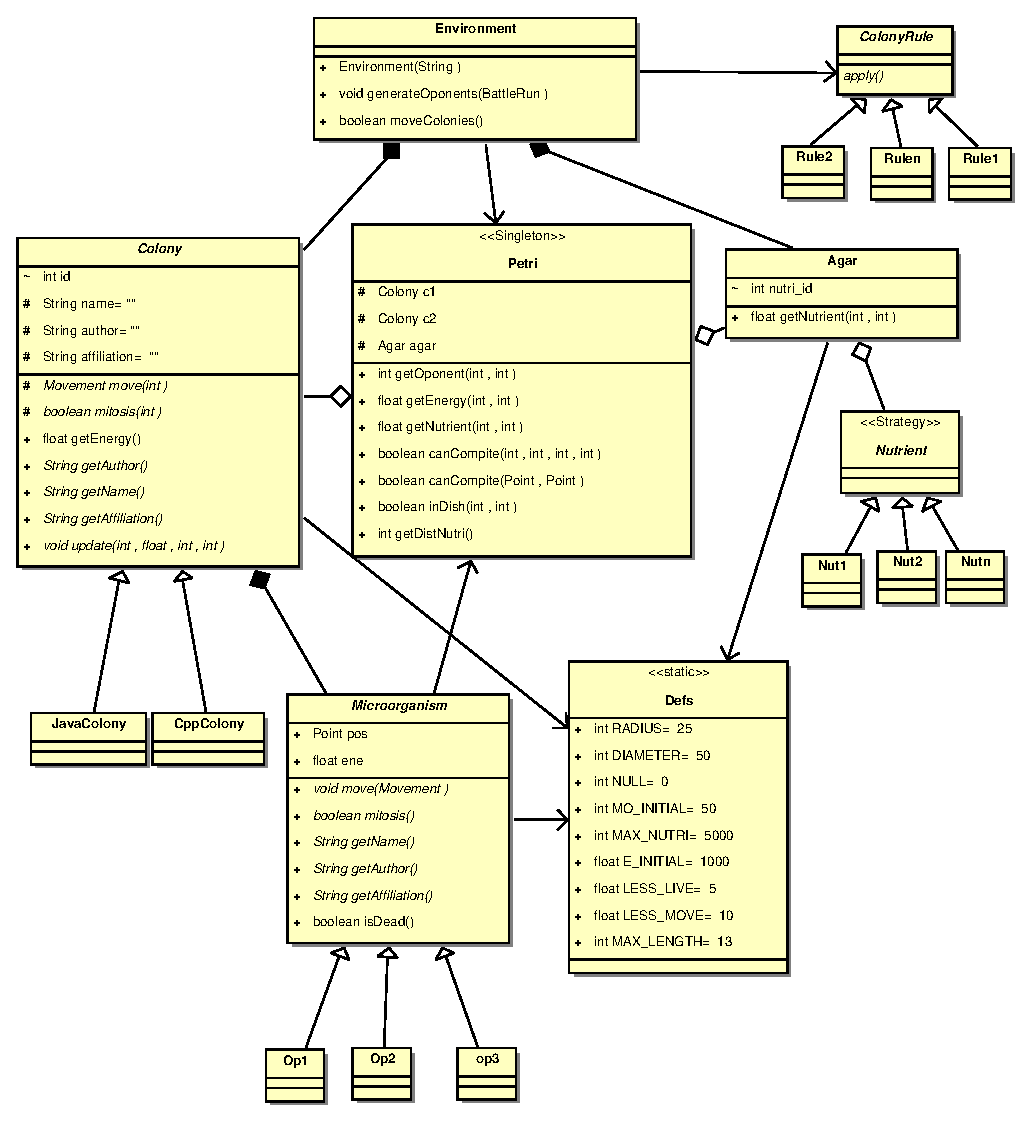
\includegraphics[scale=0.8]{modelo}

Teniendo en cuenta que el desarrollo del código es en el lenguaje Java y en base a un un Diseño Orientada a Objetos, se detallan a continuación los lineamientos generales de las clases que forman parte del programa de vida artificial.
Existe una clase a partir de la cual el concursante deberá desarrollar el método propio de supervivencia de sus microorganismos. Hay otras clases de las cuales se crearán objetos que serán de los organizadores del encuentro y que el concursante no podrá modificar. Algunos de estos objetos estarán accesibles para que los microorganismos pueden obtener datos útiles en el momento de tomar decisiones estratégicas.

El siguiente diagrama simplificado de las clases muestra el modelo del {\it Competidor1 } y del {\it Competidor2}, que son las clases de los microorganismos desarrollados por los competidores a partir de los cuales se realizarán las colonias. El método más importante es {\bf move}. El alimento para los MO es administrada por la clase {\bf Agar} y la determinación de las relaciones entre los microorganismos y su supervivencia las resuelve {\bf Environment}.

\subsection{La clase Microorganism}
\begin{center}
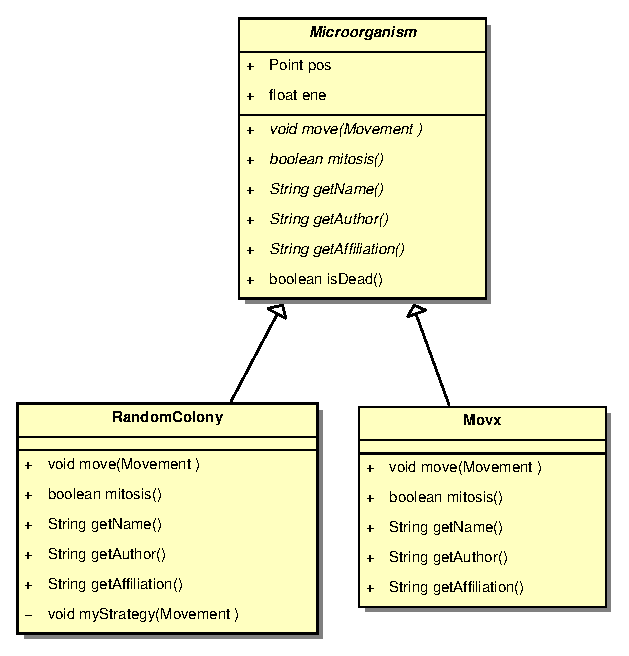
\includegraphics[scale=0.6]{microorganism}
\end{center}

Esta clase declara los métodos básicos del comportamiento, de la cual deberá heredar el MO concursante. 

En la clase descendiente que debe desarrollar el concursante, a través del método {\bf move} le indicará a donde quiere moverse cuando sea su turno.
Cuando la colonia invoca el método {\bf mitosis} del microorganismo, este indica si se quiere dividir en dos. El método {\bf update} es desde donde recibe el identificador (id) con el cual está compitiendo, sus coordenadas y energía antes de pedir que devuelva el movimiento deseado, es decir que estos atributos del MO le son informados. Este método {\bf update} es implementado únicamente en la clase madre {\bf Microorganism} por lo que no es necesario que el competidor lo redefina en su MO.

\subsection{La Clase Colony}
\begin{center}
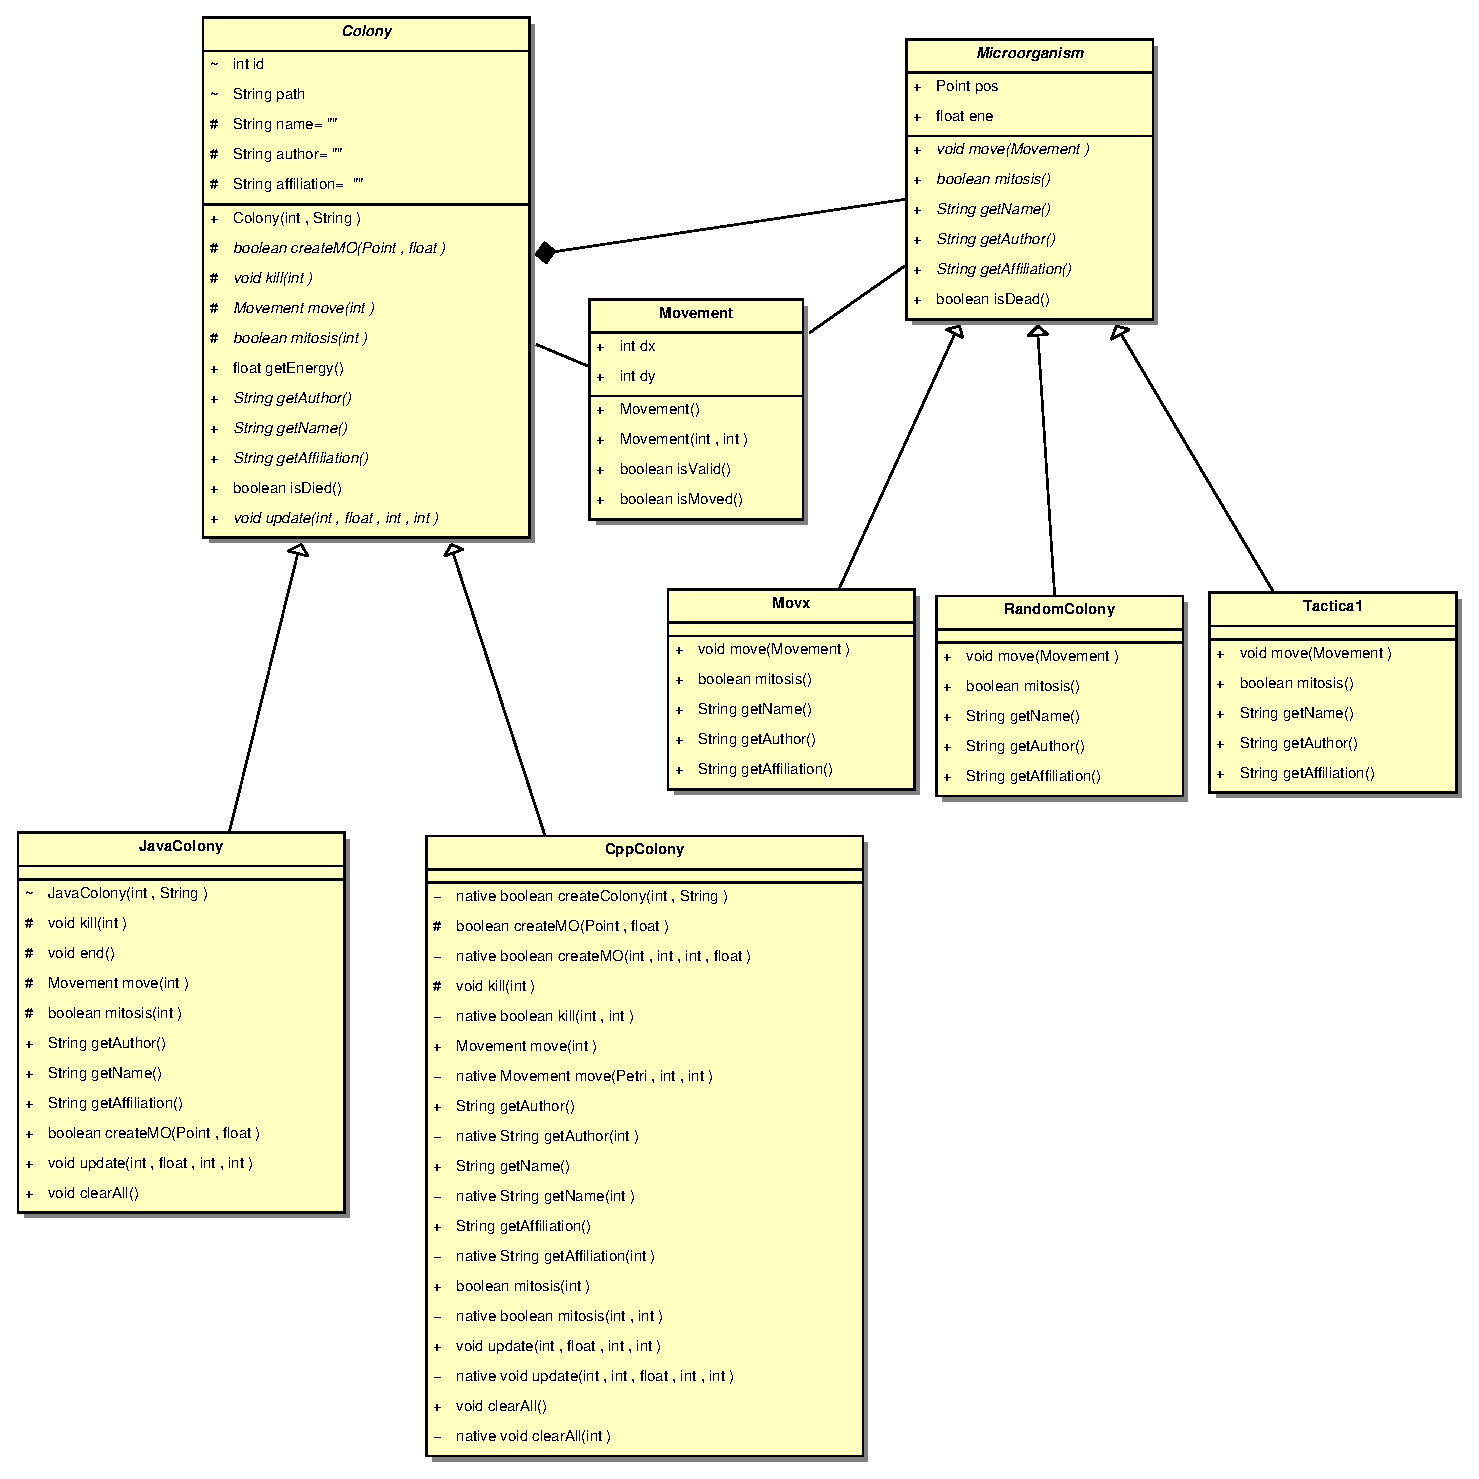
\includegraphics[scale=0.6]{colony}
\end{center}

Modela una colonia de microorganismos. Cada colonia de microorganismo puede estar implementada tanto en C/C++ como en Java. Inicialmente cada participante tiene, en su colonia, 50 microorganismos que luego pueden ir duplicándose (mitosis) e incrementando el número de microorganismos; estos también pueden morir. 

\subsection{La Clase Agar}
\begin{center}
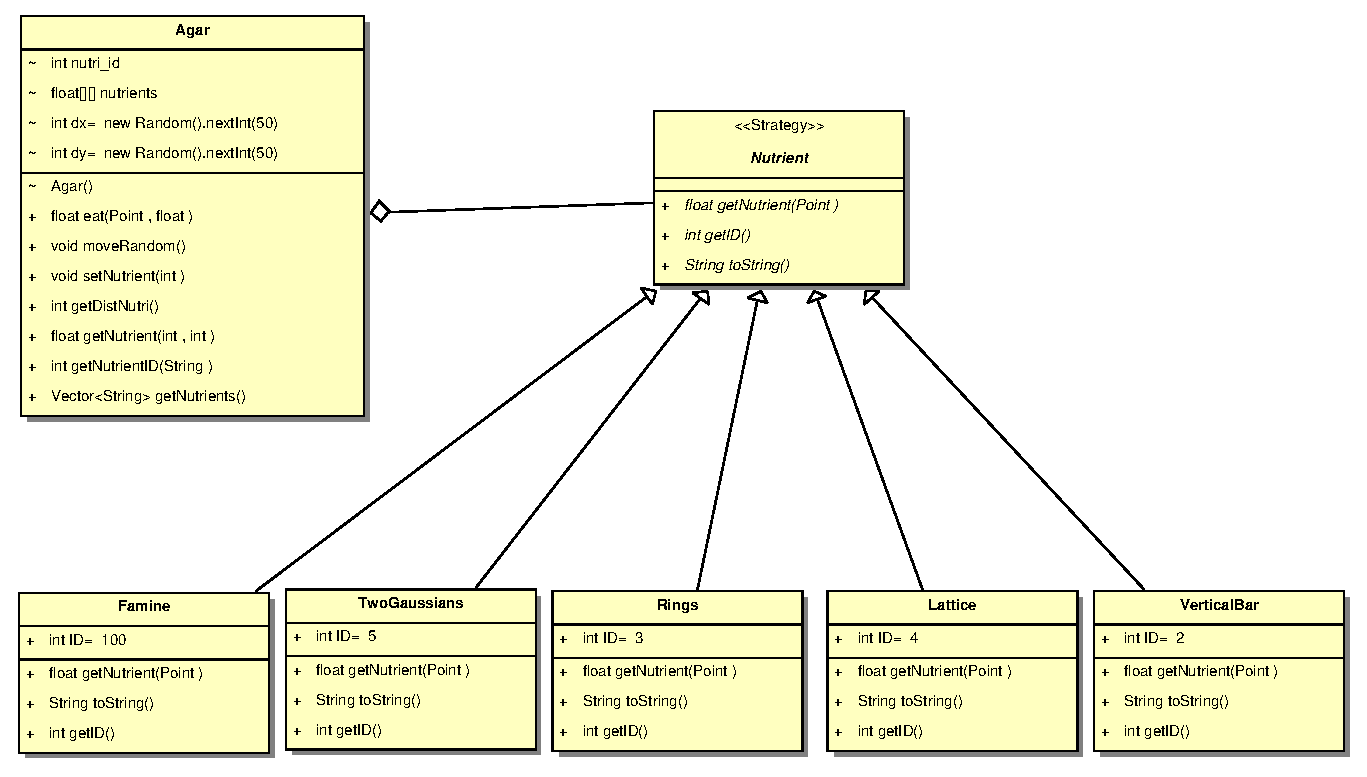
\includegraphics[scale=0.6]{agar}
\end{center}

Esta es una clase muy importante. El agar es el medio de cultivo del que se alimentan los MO y por ende es la clase que administra las distribuciones de nutrientes. 

\subsection{La Clase Petri}
\begin{center}
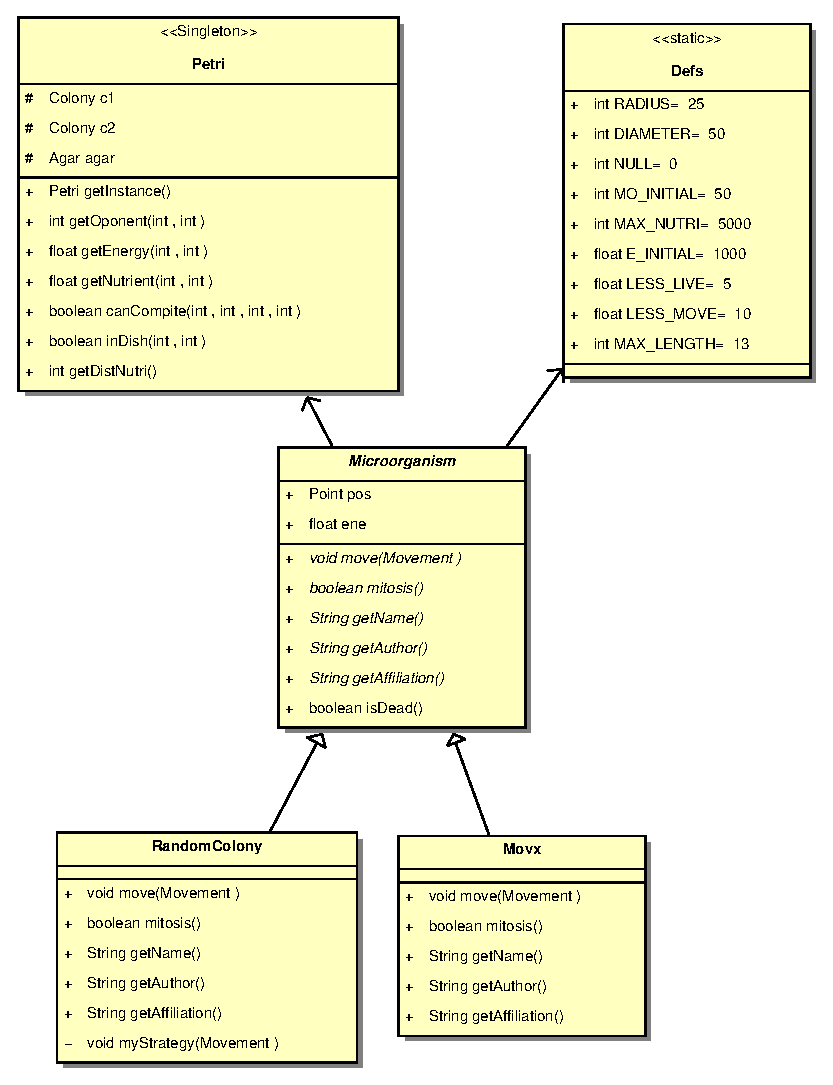
\includegraphics[scale=0.6]{petri}
\end{center}

Esta es la clase más importante para el competidor por que es la encargada de brindar información a los microorganismos. Cada competidor puedo invocarla para obtener información necesaria para tomar decisiones estratégicas. Los métodos disponibles son:

{\bf int getOponent(int x, int y):} Retorna un identificador de la clase del MO que se encuentra en la posición (x,y). si la posición está libre se retorna 0.

{\bf float getEnergy(int x, int y):} Retorna la energía del MO que se encuentra en la posicion (x,y). si la posición está libre se retorna 0.

{\bf float getNutrient(int x, int y):} Retorna la cantidad de nutrientes que hay en la posición (x, y).

{\bf int getDistNutri():} Retorna un identificador único que representa la distribución de nutrientes actual que se utiliza en una batalla.

Además, la clase Petri provee dos métodos para facilitar la programacion de un MO:

{\bf boolean canCompite():} retorna true si el MO en la posición (x1,x2) es oponente del MO en la posicion (y1,y2).

{\bf boolean inDish():} retorna true si el MO en la posición (x,y) esta dentro del entorno, es decir, pertenece al círculo del centro (Defs.Radious, Defs.Radious) y radio Defs.Radious. Defs es una clase que define las constantes importantes para la competencia, por ejemplo: cantidad de energía inicial de cada MO  ( E\_INITIAL),  radio del entorno (RADIOUS), cantidad de MOs que se crean al inicio de la competencia (MO\_INITIAL), entre otras

\section{Entorno de la competencia}

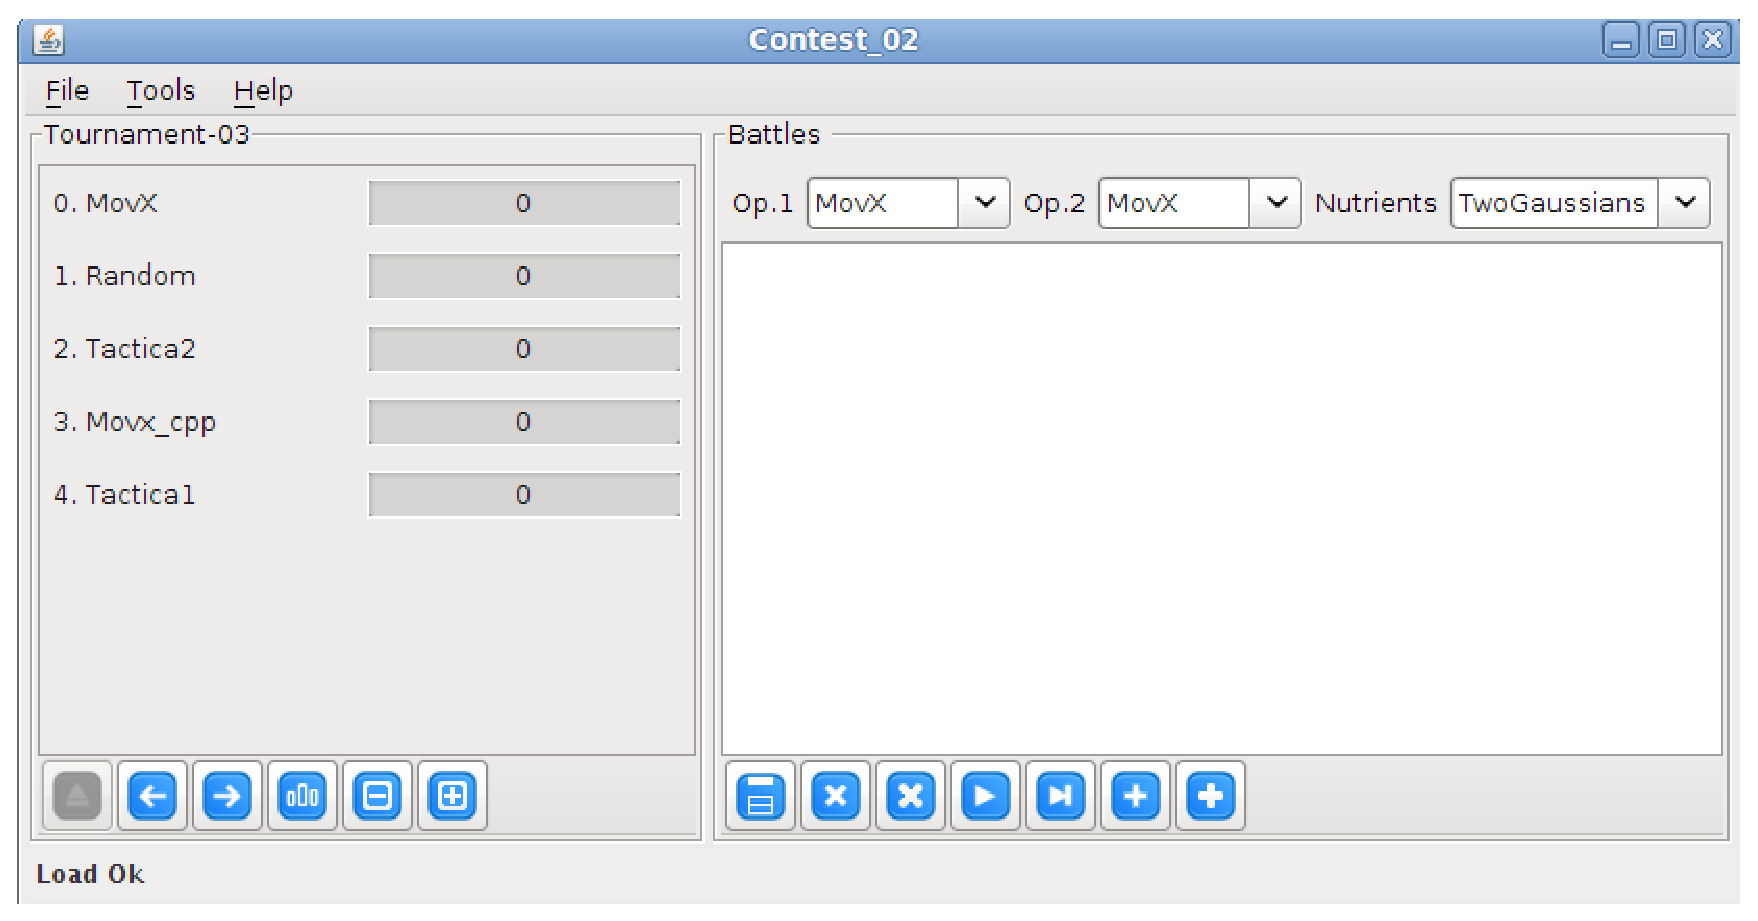
\includegraphics[scale=0.5]{frameppal}\\


Se divide en dos paneles que permiten administrar las batallas y los torneos de forma sencilla. Además posee un menú con algunas opciones y configuraciones:

{\bf Panel de torneos:} visualiza el nombre de cada colonia oponente y su respectiva energía acumulada en dicho torneo. En la parte inferior hay una lista de botones que permiten: agregar/eliminar una nueva colonia, navegar los torneos, visualizar el ranking, agregar/eliminar algún torneo.

{\bf Panel de batallas:} permite crear y ejecutar batallas en el torneo actual. Se pueden seleccionar (usando las listas selecionables que están en la parte superior del panel) los oponentes y distribución de nutrientes, y a continuación usar el botón ``agregar batalla seleccionada'' para agregar una batalla. También se puede usar el botón ``agregar todo'' para agregar las batallas que aún no se han agregado a la lista.
Para correr las batallas hay dos opciones: {\it run} y {\it run all}, donde {\it run} corre la batalla seleccionada y {\it run all} las ejecuta secuencialmente a todas y cada una.

{\bf Menu:} se divide en tres opciones (File, Tools y Help):\\
{\it Menu File:} administraciones básicas del contest.\\
{\it Menu Tools:} configuraciones(preferences) y reportes (report). En preferences se puede configurar el nombre del contest, el path del proyecto, el tiempo de pausa (en milisegundos) entre cada batalla, el modo en que corre la aplicación (programador o competencia), la distribución de nutrientes permitida en el contest y la interface gráfica que muestra las batallas.\\
{\it Menu Help:} ayuda e información del entorno. 


\subsection{¿Qué hay que saber para comenzar?}

Simplemente 2 cosas:
\subsubsection{Cómo setear los modos del entorno}
{\bf Modo programador:} está ideado para los programadores, ya que la aplicación no guarda la información respectiva a las batallas que se van realizando.

{\bf Modo competencia:} se usa solamente cuando se realizan los encuentros.

\subsubsection{Cómo hacer correr los MOs:}
Sólo hay que copiar su código en la carpeta Contest-{\it [año]}/MOs del proyecto y abrir la aplicación.

\subsection{¿Qué se debe tener en cuenta a la hora de codificar un MO?}
La clase abstracta Microorganismo es la que declara los métodos necesarios para definir el comportamiento de una colonia.
El código del concursante deberá heredarla:

\begin{lstlisting}[style=Code, language=Java]
public abstract class Microorganism {
	// Posicion absoluta del Microorganismo en el entorno.
	public Point pos;

	// Energia actual del microorganismo.
	public float ene;

	// Permite a un Microorganismo moverse a una posicion relativa de su posicion actual (pos).
	public abstract void move(Movement mov);

	// Permite a un microorganismo duplicarse.
	public abstract boolean mitosis();

	// Nombre de la colonia de Microorganismos.
	public abstract String getName();

	// Autor del codigo.
	public abstract String getAuthor();

	// Filiacion del autor del codigo!!
	public abstract String getAffiliation();
}
\end{lstlisting}

\section{Ejemplos}
\subsection{Creando un MO simple}
Supongamos que queremos crear un MO cuya táctica es moverse en forma aleatoria.
Para ello heredamos de la clase Microorganismo, como indicamos en los párrafos anteriores, e implementamos los siguientes métodos abstractos (a continuación se ejemplifica una posible implementación en el lenguaje Java):

\begin{lstlisting}[style=Code, language=Java]
//archivo RandomColony.java.

import java.util.Random;
import lib.Microorganism;
import lib.Movement;

public class RandomColony extends Microorganism{

    public void move(Movement mov) {
        // Desplazamiento aleatorio!!
        mov.dx = new Random().nextInt(3)-1;
        mov.dy = new Random().nextInt(3)-1;
    }

    public boolean mitosis() {
      // Nunca se reproduce !!
      return false;
    }

    public String getName() {
      return "Random";
    }

    public String getAuthor() {
      return "Author";
    }

    public String getAffiliation() {
     return "xxxx";
    }
}
\end{lstlisting}

\subsection{Creando un MO avanzado}
La clase Petri declara los métodos necesarios para que un MO pueda obtener información necesaria para tomar decisiones.
Los métodos que posee esta clase son los siguientes:
public Class getOponent(int x, int y) : Retorna la clase del MO que se encuentra en la posición (x,y). si la posición está libre se retorna null.
public float getEnergy(int x, int y) : Retorna la energía del MO que se encuentra en la posición (x,y). si la posición está libre se retorna 0.
public float getNutrient(int x, int y) : Retorna la cantidad de nutrientes que hay en la posición (x, y).
Además, la clase Petri provee dos métodos para facilitar la programación de un MO:
public boolean canCompite(): retorna true si el MO en la posición (x1,x2) es oponente del MO en la posición (y1,y2).
public boolean inDish(): retorna true si el MO en la posición (x,y) esta dentro del entorno, es decir, pertenece al círculo del centro (Defs.Radious, Defs.Radious) y radio Defs.Radious. Defs es una clase que define las constantes importantes para la competencia, por ejemplo: cantidad de energía inicial de cada MO(E\_INITIAL), radio del entorno (RADIOUS), cantidad de MOs que se crean al inicio de la competencia (MO\_INITIAL), entre otras.

Ahora usando la información que nos provee la Clase Petri, podemos crear un MO que realice movimientos más avanzados, por ejemplo tratando de atacar al enemigo adyacente:

\begin{lstlisting}[style=Code, language=Java]
public void move(Movement mov){
    Point p = new Point();

    for(int i; 1; i++){
        for(int j; 1; j++){
            // la posicion pos es la posicion actual del MO.
            p.x = pos.x+i;
            p.y = pos.y+j;

            if(petri.inDish(p) && petri.canCompite(pos, p)){ // me muevo a esa Posicion!!
                mov.dx = i;
                mov.dy = j;

                return;
            }
        }
    }
}
\end{lstlisting}

\section{Utilidades}

\subsection{Util.jar}
Esta utilidad permite facilitar la utilización del entorno.

\begin{enumerate}
\item {\bf Modo de uso: } en forma genérica se puede invocar a Util.jar como lo indica el ejemplo:
 \begin{lstlisting}[style=Code]
 java -jar Util.jar OPCION [PARAMETROS]
\end{lstlisting}
	donde las opciones pueden ser MO, compile o clean y los parámetros varían de acuerdo a la opción.
\item {\bf Compilar la aplicación:} el competidor puede utilizar el comando, como se muestra a continuación, para compilar y chequear la sintaxis de su código fuente (puede estar implementado tanto en el lenguaje Java como en C/C++). 
\begin{lstlisting}[style=Code]
java -jar Util.jar MO [Directorio de los MOs]/nombreMO.[java/h]
\end{lstlisting}
por ejemplo:
\begin{lstlisting}[style=Code]
java -jar Util.jar MO Contest_02/MOs/miMO.java
java -jar Util.jar MO Contest_02/MOs/miMO.h
\end{lstlisting}
\item {\bf Eliminar archivos innecesarios:} utilizando el parámetro clean se puede eliminar archivos temporales y/o de compilación que estén en el proyecto.
\begin{lstlisting}[style=Code]
java -jar Util.jar clean
\end{lstlisting}

\item {\bf Compilar el entorno: } el parámetro compile permite compilar nuevamente toda la aplicación.
\begin{lstlisting}[style=Code]
java -jar Util.jar compile
\end{lstlisting}

\end{enumerate}	 

\end{document}
 
